By this point in the analysis all the selections have been finalised and discussed.
Furthermore, clear definitions for tag-$B$ mesons that properly kinematically constrain \BtoXsgamma are presented, such that \EB is evaluated accurately.
However, as can be seen \Cref{fig:spectrum_after_optimisation}, even though continuum and $\BB$ backgrounds is suppressed heavily compared to the \EB distributions that was begun with (\Cref{fig:spectrum_after_reco}),
there is still a significantly larger number of background processes than \BtoXsgamma signal events.
Many of these, particularly continuum background, originate from incorrect tag-$B$ mesons (see \Cref{fig:good_tag_definitions}) and can therefore be estimated in data using an \Mbc fitting procedure.
In this section, a thorough overview of the \Mbc fit will be presented which will extract the counts of good-$B$ tags in different \EB intervals.

\subsection{Components in the dataset}\label{sec:fitting_components}

There are three types of events in \epem collision dataset following all the selections described so far:
\begin{itemize}
    \item Generic-\BB (including \BtoXsgamma) that are tagged with a good tag-$B$;
    \item Generic-\BB (including \BtoXsgamma) that are tagged with a misreconstructed tag-$B$;
    \item Photons candidates originating in \epem\ra\qqbar.
\end{itemize}
These three components are referred to as `peaking', `combinatorial \BB' and `continuum' throughout this \Cref{sec:fitting_mbc}.
These components, extracted from generic \MC, are visualised in \Cref{fig:tag_component_fits}.

\begin{figure}[htbp!]
    \centering
    \subcaptionbox{\label{fig:good_tags_fit}}{
        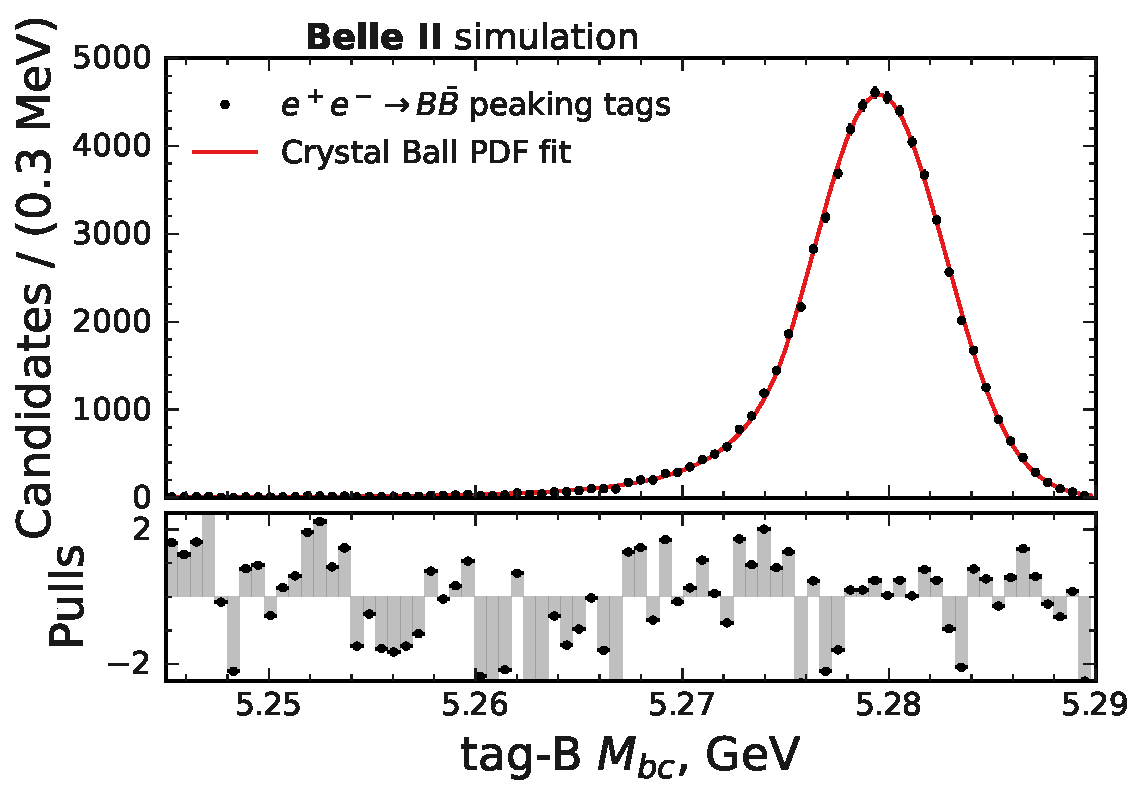
\includegraphics[width=0.3\textwidth]{figures/fitting/mbc_good_tags_fit.pdf}
    }
    \subcaptionbox{\label{fig:combinatorial_tags_fit}}{
        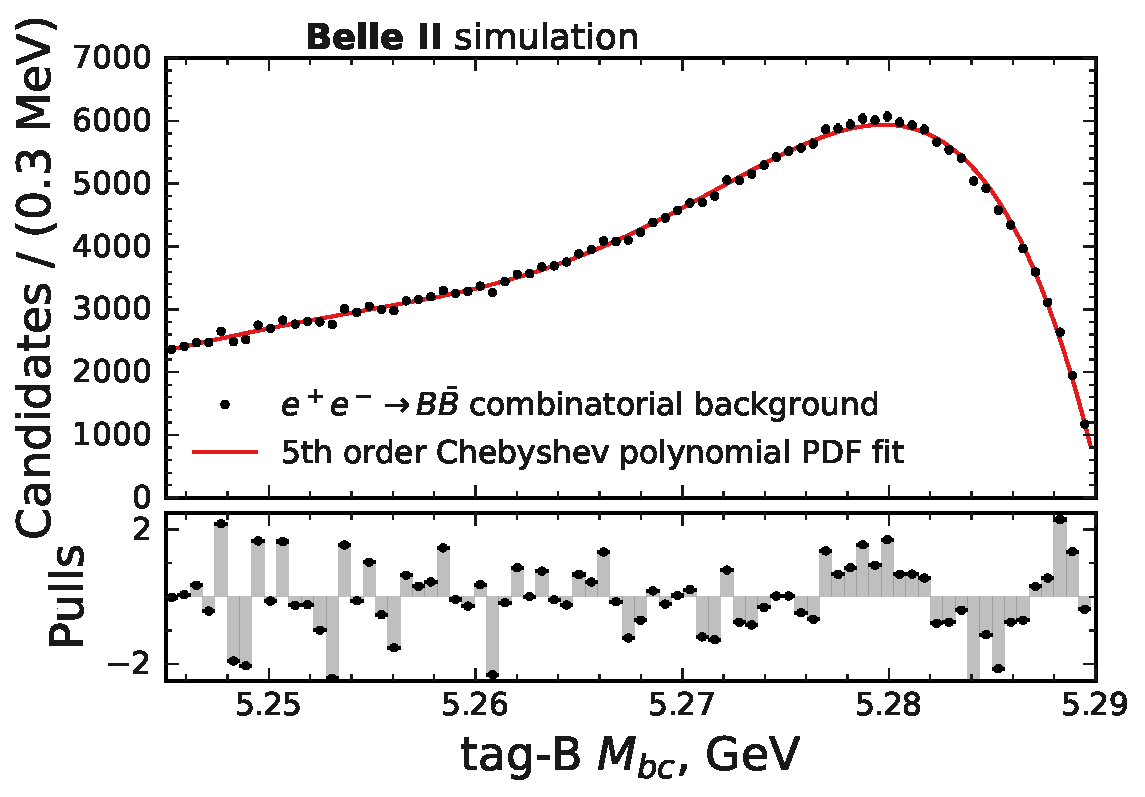
\includegraphics[width=0.3\textwidth]{figures/fitting/mbc_combinatorial_tags_fit.pdf}

    }
    \subcaptionbox{\label{fig:argus_tags_fit}}{
        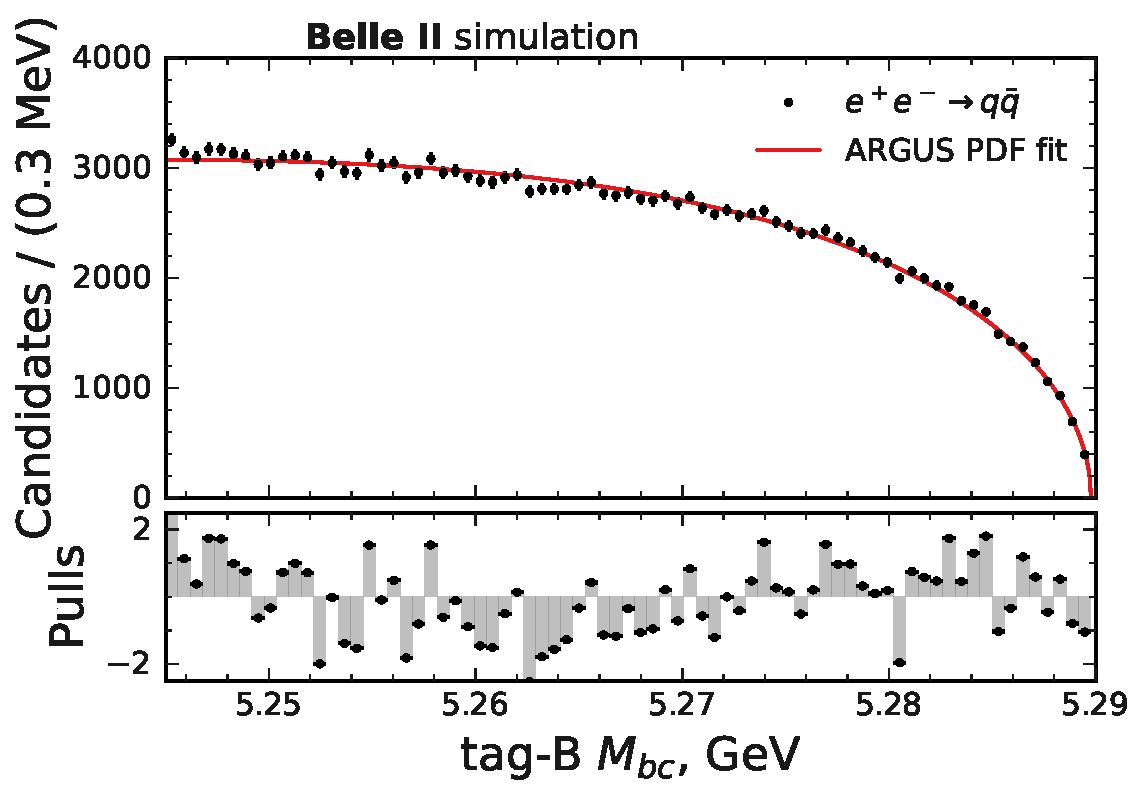
\includegraphics[width=0.3\textwidth]{figures/fitting/mbc_continuum_tags_fit.pdf}
    }
    \caption{\label{fig:tag_component_fits} Separate components that are present in generic \MC after selections that suppress background (\Cref{tab:cutflow}).
    The individual components are defined in \Cref{sec:fitting_components} text.
    Each distribution contains an unbinned illustrative fit to the data points, and the subpanels show the pull (\Cref{eq:pull_distribution}) in each case.
    The fitting function for peaking tag \B mesons (\Cref{fig:good_tags_fit}) is chosen as the Crystal Ball function;
    for combinatorial tag \B mesons (\Cref{fig:combinatorial_tags_fit}) it is chosen as the 5th order Chebyshev;
    for continuum \epem\ra\qqbar events (\Cref{fig:argus_tags_fit}) it is chosen as the ARGUS function.
    }
\end{figure}

The fitting model is prepared to describe the three components and, particularly, to extract the number of tag-$B$ candidates that corresponds to the `peaking' component.
The strategy to describe each component is as follows:
\begin{itemize}
    \item Peaking \Mbc distributions are often fitted using a Crystal Ball function.
    It is defined in \Cref{sec:crystal_Ball}, but can be understood as Gaussia distribution with a polynomial tail.
    \Cref{fig:good_tags_fit} illustrates the suitability to describe the peaking \Mbc distribution.
    \item Continuum \Mbc distributions are conventionally described by the ARGUS function, which is named after the ARGUS collaboration and designed specifically for this purpose;
    This function, utilised to describe \epem\ra\qqbar simulated backgrounds in this analysis is seen in \Cref{fig:argus_tags_fit}.
    \item The particular shape of the combinatorial \BB background is generally dependant on the signal mode and do not have a conventional method of description.
    In this analysis, the usage of \FEI and the fact that background events are conservatively suppressed to avoid signal-side biases leads to an wide but slightly peaking shape.
    Several options were assessed in this ana;lysis, but it was found that it is suitably described by a Chebyshev polynomial, which can be adapted to a necessary functional shape.
    This is illustrated in \Cref{fig:combinatorial_tags_fit}, where a 5th order polynomial describes the combinatorial \BB background distribution.
\end{itemize}
In \Cref{fig:tag_component_fits} the subpanels shown the pull distribution, which is defined as:
\begin{equation}\label{eq:pull_distribution}
    \mathrm{pull}(x) = \frac{x-\mu}{\sigma}. 
\end{equation}
Throughout this thesis it is used to evaluate the quality of the fit, as repeated measurements of a random variable $x$ should fluctuate around a mean value $\mu$ with a possonian width $\sigma$.
Therefore any dependancies or strucutes observed in the pull distribution would be indicators of poor fit quality. 

\subsection{Photon energy intervals for the fit}\label{eq:binning}

The final goal of the analysis is to extract he photon energy spectrum.
Performing the \Mbc fit with \PDF{s} described in \Cref{sec:fitting_components} in different \EB bins can provide the number of good-tags in each \BB bin.

It is clear from \Cref{fig:spectrum_after_optimisation} that there are different signal-to-background ratios accross all \EB range.
However, it can also be seen that generall signal-to-\BB-event ratios and signal-to-continuum ratios are also changing.
In order to ensure appropriate signal extraction